\title{Note on error analysis of the extracted time resolution using the automated 6-bar analysis program}
\date{January 18, 2015}

\documentclass[12pt]{article}

\usepackage{hyperref}
\usepackage{cite}

\usepackage{graphicx}
%\usepackage{epsfig}
\usepackage{epstopdf}

\usepackage{mathtools}
\newcommand{\defeq}{\vcentcolon=}

\usepackage{float}
\restylefloat{table}

%! To create a place-holder figure
\newcommand{\dummyfig}[1]{
  \centering
  \fbox{
    \begin{minipage}[c][0.33\textheight][c]{0.5\textwidth}
      \centering{#1}
    \end{minipage}
  }
}

\begin{document}
\maketitle

% \begin{abstract}
% This is the paper's abstract \ldots
% \end{abstract}

\section{III.E. Photomultiplier tubes (PMTs)}

\subsection{Different PMTs time resolutions}
\textit{My assumptions in writing this section}
\begin{enumerate}
	\item \textit{Our chosen PMT(R9779) was compared with panel-1a PMT(EMI9954A)}
	\item \textit {Details of relevant differences of the tech-specs of the two PMTs and therefore the expected superiority of R9779 over EMI9954A will be listed elsewhere; here we will only give empirical proof}
\end{enumerate}

The selected Hamamatusu's R9779 PMTs for panel-1b were compared with Electron Tubes EMI 9954A in the 3-bar setup (\textit{I am assuming that the 3-bar setup will either already be defined or referred to in another publication, so as to not go into details, but simply for the reader to trust that it is our way to extract time-resolution, though, it is NOT directly the time-resolution of the PMT, but of the entire counter; this is important to keep in mind, since for the old TOF system, PMT resolutions were directly compared using lasers; details of this method are in old CLAS-SC NIM paper.})

\textit{Should I mention here that for EMI PMT tests, the contribution of the LFIO module was removed?}

Below is the figure that shows the superiority of the R9779:
\begin{figure}[th]
	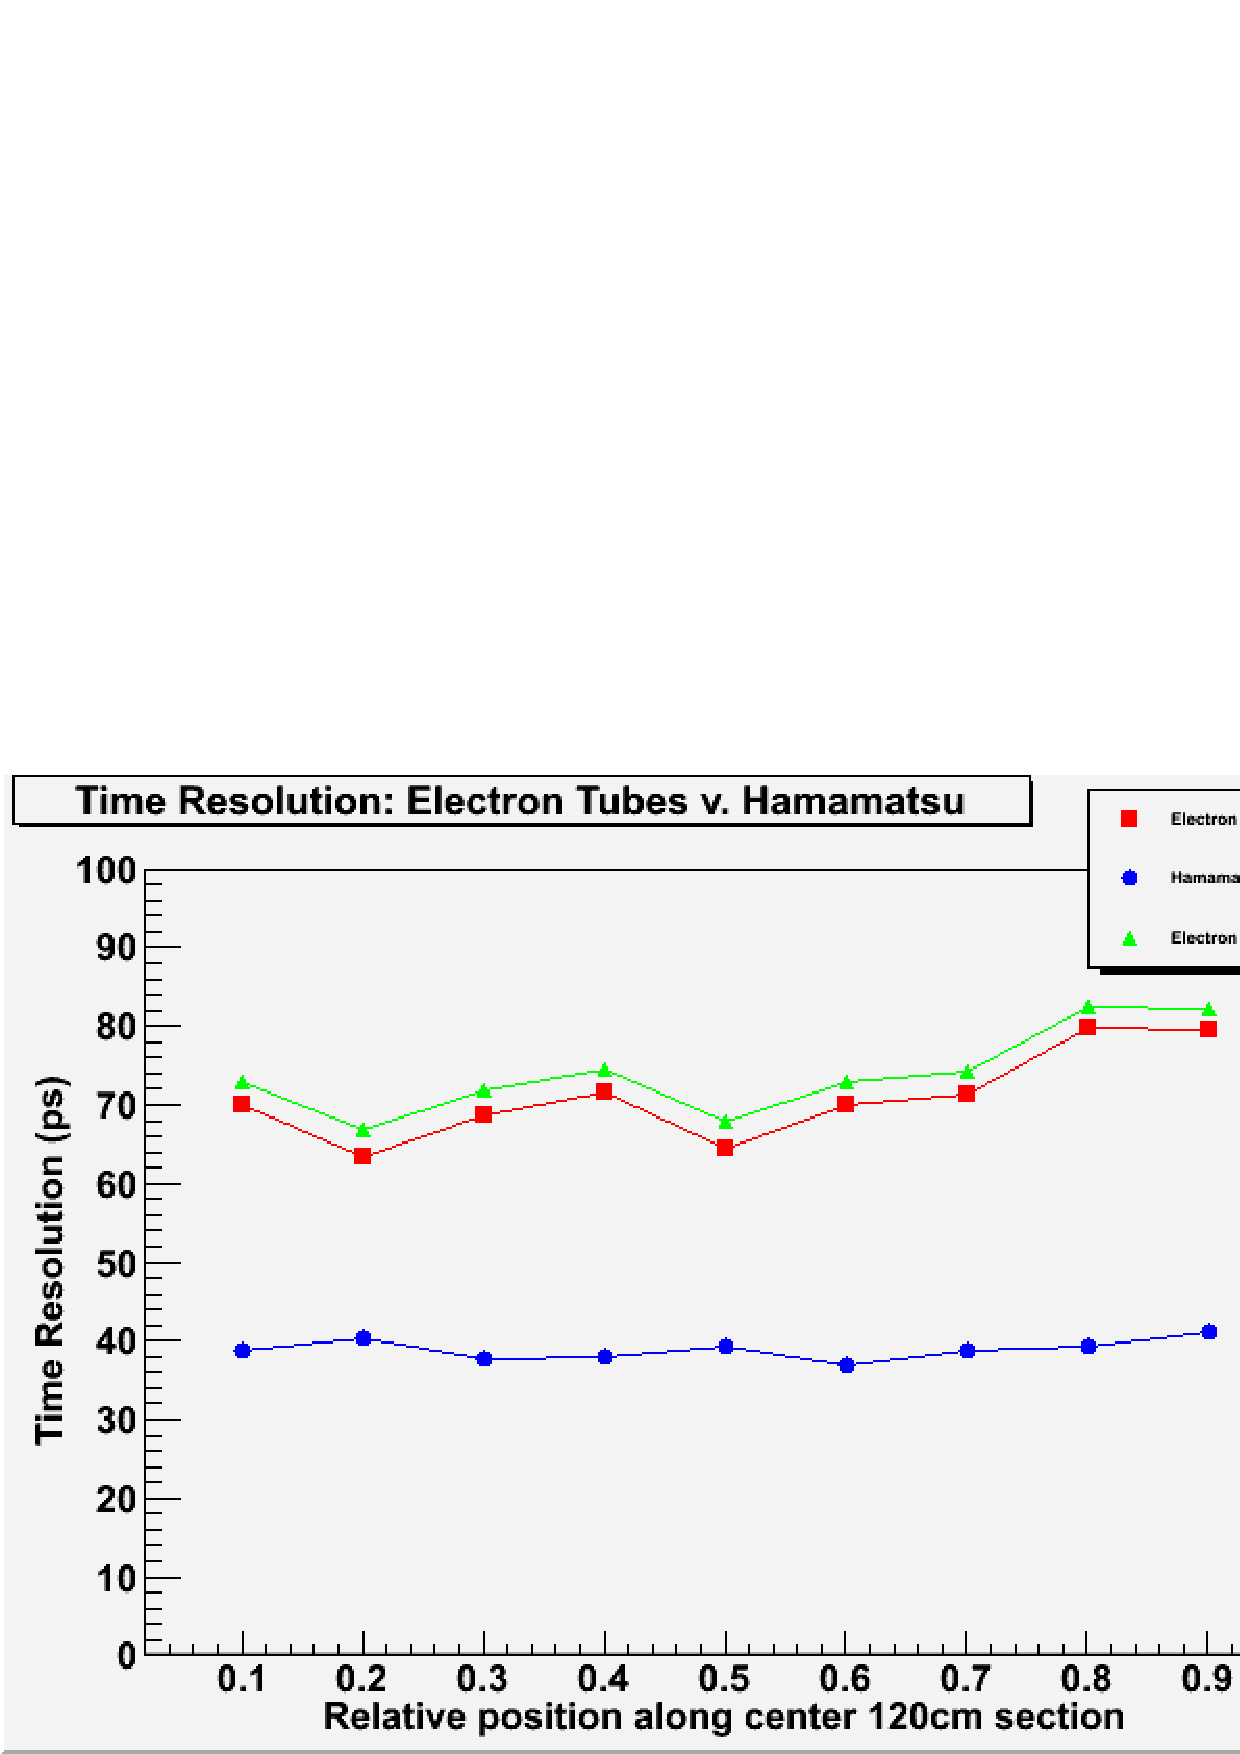
\includegraphics[width=10cm, height=5cm]{PMTcomparison.pdf}
\end{figure}

\subsection{... threshold dependence}
We also compared various threshold (\textit{Define "threshold"}) levels for the signals from the PMT and see if it had any affect on the time resolution. The threshold levels tried were:50mV, 75mV, 150mV, 300mV, and 600mV.

Following is a figure that demonstrates varying the threshold did not affect the time resolution.
\begin{figure}[th]
	\includegraphics[width=10cm, height=5cm]{ThresholdsTimeRes.pdf}
\end{figure}

\section{III.G. Magnetic shielding of the PMTs}
The photomultipliers that are attached to the FTOF scintillators will be exposed to the combined stray magnetic fields from the CLAS12 solenoid and torus magnets. It is therefore important to study the effect of the magnetic field strength on the anode signal of a PMT and ultimately on the time resolution of the FTOF detector system. In the experimental test setup, a PMT was set on a flat, non-magnetic base in between a pair of Helmholtz coils and the anode signal of the PMT was digitized and processed by a DAQ system . This arrangement is shown in Fig. 1.

\begin{figure*}[ht]
  \includegraphics[width=2.5in]{placeholder.pdf} 
  \caption{PMT B field test setup}
  \label{fig1}
\end{figure*}

Due to the dynode-array geometry of the PMT and the electrodynamic processes which finally contribute to the signal formation, the studies need to be performed in dependence of the orientation of the PMT relative to the magnetic field. Given the axial Helmholtz magnetic field, the orientation of a PMT in it can be described by two rotational degree of freedoms; their axes are illustrated in Fig. 2 and defined by the PMT's axis of cylindrical symmetry, $\hat{z}$ and the radial axis perpendicular to $\hat{z}$ and horizontal to the flat base supporting the PMT, $\hat{\rho}$.

In the axial Helmholtz magnetic field, a PMT can be rotated around $\hat{\rho}$ until $\hat{z}$ is aligned transversely (T) or longitudinally (L) with the field direction. These are the two orientations in which a PMT is observed to have the two strongest and in a sense, independent responses; any other orientation is dominated by a superposition of the two responses. These two orientations are illustrated in Fig. 2.

\begin{figure*}[ht]
  \includegraphics[width=2.5in]{placeholder.pdf} 
  \caption{Tranverse and longitudnal orientations of PMT in axial B field}
  \label{fig2}
\end{figure*}

The additional change in the signal response of a PMT when it was rotated around $\hat{z}$ was also studied, primarily when it is already aligned in the transverse orientation (minimal to no effect due to rotations around $\hat{z}$ is observed in the longitudinal orientation) \cite{Steinman} However, after implementing the final shielding configuration (see Sec. 2.2), the PMT response no longer depends on the rotational degree of freedom around $\hat{z}$.

It is worth mentioning here that the magnetic field primarily affects the signal amplitude, while the signal shape and smoothness, which have a far larger impact on the time resolution, are mostly unaffected \cite{Steinman}. However, the loss of signal amplitude does affect the extracted time resolution, but only when the reduction reaches levels at which the Time-walk corrections become less efficient. Therefore, the signal reduction level was used as the parameter to quantify the response of a PMT in a magnetic field and its affect on the time resolution. 

Even though it was established that when the signal amplitude is reduced by 10\% in the longitudinal and the transverse orientations there is no change in the time resolution - measured to be $41\;ps$ and $38\;ps$, respectively ($39\;ps$ with no magnetic field) \cite{Steinman} -  the final design of the magnetic shielding (Sec. 2.2) is such that up to magnetic field strengths higher than those expected in CLAS12, the signal amplitude shows no reduction; the maximum stray field strength that the panel-1b PMTs are going to be exposed to is expected to be 22G at counters placed at the largest angular extent of the FTOF12 detector system, of which 2/3 (15G) will be in the axial direction \cite{CLAS12FTOFstudies} and the tests at USC were done with magnetic fields up to 30G, wholly directed in either the transverse or longitudinal directions.

\subsection{Initial design considerations}
The PMT assemblies R9779-20MOD are already manufactured with a layer of mu-metal coating. It can be seen from Tab. 1 that in the transverse orientation, compared to a PMT without any mu-metal coating, the inbuilt mu-metal shielding preserves the signal amplitude to much higher levels of magnetic fields.

\begin{table}[H]
	\begin{center}
		\begin{tabular}{|c|c|l|}
			\hline
	 		& no mu-metal & with mu-metal \\
			\hline
 			10G-L & 10\% & 10\% \\
 			10G-T & 100\% & 0\% \\ 
 			\hline
 			15G-L & XX\% & XX\% \\
 			15G-T & 100\% & 0\% \\
 			\hline
 			15G-L & YY\% & YY\% \\
 			15G-T & 100\% & 0\% \\
 			\hline
 			20G-L & ZZ\% & ZZ\% \\
 			20G-T & 100\% & 10\% \\
 			\hline
 			25G-L & AA\% & AA\% \\
 			25G-T & 100\% & XX\% \\
 			\hline
 			30G-L & BB\% & BB\% \\
 			30G-T & 100\% & BB\% \\
 			\hline
		\end{tabular}
	\end{center}
	\caption{Reduction of PMT anode signal in various test configurations}
\end{table}


However, even with the inbuilt mu-metal shielding, there is a rapid deterioration of the signal past 10G-L and XXG-T and this led to considering further shielding methods.

\subsubsection{External shielding}
In order to provide additional shielding, a rectangular external mu-metal shielding, with each side of thickness $2\;mm$, was designed. Tab. 2 shows that within this external shielding, in the transverse orientation, the signal amplitude is preserved up to $30\;G$. However, this provided no additional protection to PMT in the longitudnal orientation.

\begin{table}[H]
	\begin{center}
		\begin{tabular}{|c|c|}
			\hline
	 		& external mu-metal shielding \\
			\hline
 			10G-L & 10\% \\
 			10G-T & 0\% \\ 
 			\hline
 			15G-L & XX\% \\
 			15G-T & 0\% \\
 			\hline
 			15G-L & YY\% \\
 			15G-T & 0\% \\
 			\hline
 			20G-L & ZZ\% \\
 			20G-T & 0\% \\
 			\hline
 			25G-L & AA\% \\
 			25G-T & 0\% \\
 			\hline
 			30G-L & BB\% \\
 			30G-T & BB\% \\
 			\hline
		\end{tabular}
	\end{center}
	\caption{Signal reduction of PMT's anode signal in presence of external mu-metal shielding. It is observed that PMT signal's reduction is unchanged in the longitudinal orientation, but the signal is preserved to $30\;G)$ in the transverse orientation}
\end{table}

\subsection{Final implementation of shielding with overhang}
To also preserve the signal amplitude in the longitudinal orientation, it was decided that in the final implementation, the external shielding would extend a few centimeters beyond the front face of the PMT ($\defeq$ overhang). This requires shaving two edges of the scintillator bars by a few millimeters. Tab. 4 shows the results of testing the signal reduction at various overhang positions of the external shielding. The overhang position of $4\;cm(1.5\;in)$ is sufficient to preserve the signal up to $30\;G$ in the longitudinal orientation.

\begin{table}[H]
	\begin{center}
		\begin{tabular}{|c|c|c|c|c|c|}
			\hline
	 		& $0\;cm$-overhang & $1\;cm$-overhang & $2\;cm$-overhang & $3\;cm$-overhang & $4\;cm$-overhang \\
			\hline
 			10G-L & & & & & \\
 			10G-T & & & & & \\ 
 			\hline
 			15G-L & & & & & \\
 			15G-T & & & & & \\
 			\hline
 			15G-L & & & & & \\
 			15G-T & & & & & \\
 			\hline
 			20G-L & & & & & \\
 			20G-T & & & & & \\
 			\hline
 			25G-L & & & & & \\
 			25G-T & & & & &\\
 			\hline
 			30G-L & & & & & \\
 			30G-T & & & & & \\
 			\hline
		\end{tabular}
	\end{center}
	\caption{Signal reduction of PMT's anode signal in presence of external mu-metal shielding at various overhang positions. It is observed that at the overhang position of $4\;cm$ the signal is preserved up to magnetic field strength of $30\;G$ in both the transverse and longitudinal orientations}
\end{table}


\section{Establishing an upper limit on the level of tolerable magnetic field} In the final design and implementation of the magnetic shielding, the tests show that there is going to be no reduction in signal amplitude in fields up to $30\;G$ in the transverse and longitudinal orientation. This is already beyond the maximum fields to which the PMTs will be exposed to according to the CLAS12 design requirements \cite{CLAS12FTOFstudies}. However, tests were run to note signal reduction levels as the magnetic field strength was increasted beyond $30\;G$ in each of the orientations and the point at which the signal amplitude reduced by 10\% in each of the orientations, transverse and longitudinal, was noted. Since up to such reduction levels, the time resolution is unaffected, the noted field strength serves as the conservative upper limit of the magnetic field at which the time resolution remains unaffected. Tab. 4 shows the results of such tests which establishes the conservative upper limit at $XX\;G$ and $YY\;G$ in the transverse and longitudinal orientations, respectively.

\begin{table}[H]
	\begin{center}
		\begin{tabular}{|c|c|}
			\hline
			30G-L &  \\
 			30G-T &  \\ 
 			\hline
 			35G-L &  \\
 			35G-T &  \\
 			\hline
 			40G-L &  \\
 			40G-T &  \\
 			\hline
 			45G-L & \\
 			45G-T &  \\
 			\hline
 			50G-L &  \\
 			50G-T &  \\
 			\hline
 		\end{tabular}
	\end{center}
	\caption{Signal reduction of PMT's anode signal beyond the design consideration of $30\;G$}
\end{table}


\subsection{Results and Conclusions}
With the finally designed and implemented shielding, the time resolution of the panel-1b FTOF counters remains unaffected by the presence of fringe magnetic fields in CLAS12 up to a field level of at least $XX\;G$ and $YY\;G$ in the transverse and longitudinal orientations, respectively. This exceeds the maximum field of $22\;G$ (of which 2/3 will be in longitudinal direction) to which the panel-1b PMTs are expected to be exposed to. 



% \phantomsection
% \addcontentsline{toc}{chapter}{Bibliography}
\label{bib}
\bibliographystyle{abbrv}
\bibliography{at_contrib}

\end{document}